\documentclass[11pt,letterpaper]{article}
\usepackage{tikz}
\usepackage{comment}
\usepackage{xcolor}
\usepackage[backend=biber, style=ieee]{biblatex} 
\addbibresource{midterm_report/assets/refs.bib}
\usepackage[utf8]{inputenc}
\usepackage{graphicx}
\usepackage{float}  
\usepackage{fullpage}
\usepackage{subcaption}
\usepackage{listings}
\usepackage{xcolor}
\usepackage{wrapfig}



% Define code style
\lstdefinestyle{pythonstyle}{
    backgroundcolor=\color{gray!10},   % Background color
    commentstyle=\color{green},        % Comment style
    keywordstyle=\color{blue},         % Keyword style
    numberstyle=\tiny\color{gray},     % Line numbers style
    stringstyle=\color{orange},        % String style
    basicstyle=\ttfamily\footnotesize, % Basic font style
    breaklines=true,                   % Line breaking
    frame=single,                      % Frame around the code
    numbers=left,                      % Line numbers on the left
    captionpos=b,                      % Caption at the bottom
    showstringspaces=false             % Hide spaces in strings
}

\lstset{style=pythonstyle}

\begin{document}


\title{DeClip: Removing key components }


\author{
Zhanhao Liu (zhanhaol@umich.edu),
Huanchen Jia (jhuanch@umich.edu),\\
Qiulin Fan (rynnefan@umich.edu),
Lingyu Meng (jmly@umich.edu)\\
}

\date{03/14/2025}


\maketitle

\section{Abstract}
Contrastive Language–Image Pretraining excels in multimodal learning, enabling zero-shot classification, cross-modal retrieval, and transfer learning. However, its reliance on global image-text alignment limits its ability to capture localized features, weakening performance in fine-grained visual tasks. To address this, DeClip introduces image-based hard negatives by modifying key image-caption pairs, enhancing model robustness and discrimination. This improves CLIP’s ability to distinguish fine-grained details, strengthening its effectiveness in contrastive learning and multimodal tasks.

\section{Introduction}
CLIP\cite{radford2021learningtransferablevisualmodels} (Radford et al., 2021), trained on full images, struggles to learn localized features due to its reliance on global image-text alignment, limiting its effectiveness in fine-grained visual-text tasks like object classification and caption-based retrieval. This limitation hinders its ability to capture subtle visual differences, which is especially problematic in safety-critical domains such as medical imaging and robotics, where precise distinctions—like identifying diseased tissue or ensuring accurate tool positioning—are crucial. Solving this problem would improve CLIP’s ability to learn localized visual details, enhancing its adaptability to tasks requiring fine-grained reasoning and ultimately making it more effective in real-world multimodal applications.
    



% While CLIP effectively aligns high-level semantics, its dependence on global cues can obscure fine-grained details crucial in safety-critical domains like medical imaging, robotics, and autonomous systems, where minute differences—such as distinguishing healthy from diseased tissue or detecting precise object orientations for robotic grasping—can have significant consequences. By training models with DeClip, we aim to enable them to learn localized features and capture positional and orientation cues, though further validation is required to refine and assess this capability.



\section{Proposed method}
\subsection{Overall Approach}
Prior research suggests that, for each pair of correct (image, caption) example, by rewriting the caption, e.g. reordering and changing its constituents, we can generate into a very hard negative. (Fan, Krishnan, et. al.\cite{fan2023improvingcliptraininglanguage}). Our idea has similarities and extensions. We propose another idea to mine hard negaives on the image side. For each true example in a subset of the dataset, we remove some key components from the image and keep the rest, leave the resulting image a high degree of similarity to the original image, but does not fit the caption, as a hard negative. We then dually remove the keywords on the caption, as a new positive example.

For the new image after removing the keyword, we call it \textbf{dual image}; for the new caption after removing the keyword, we call it \textbf{dual text}. 

\begin{figure}{H}
    \centering
    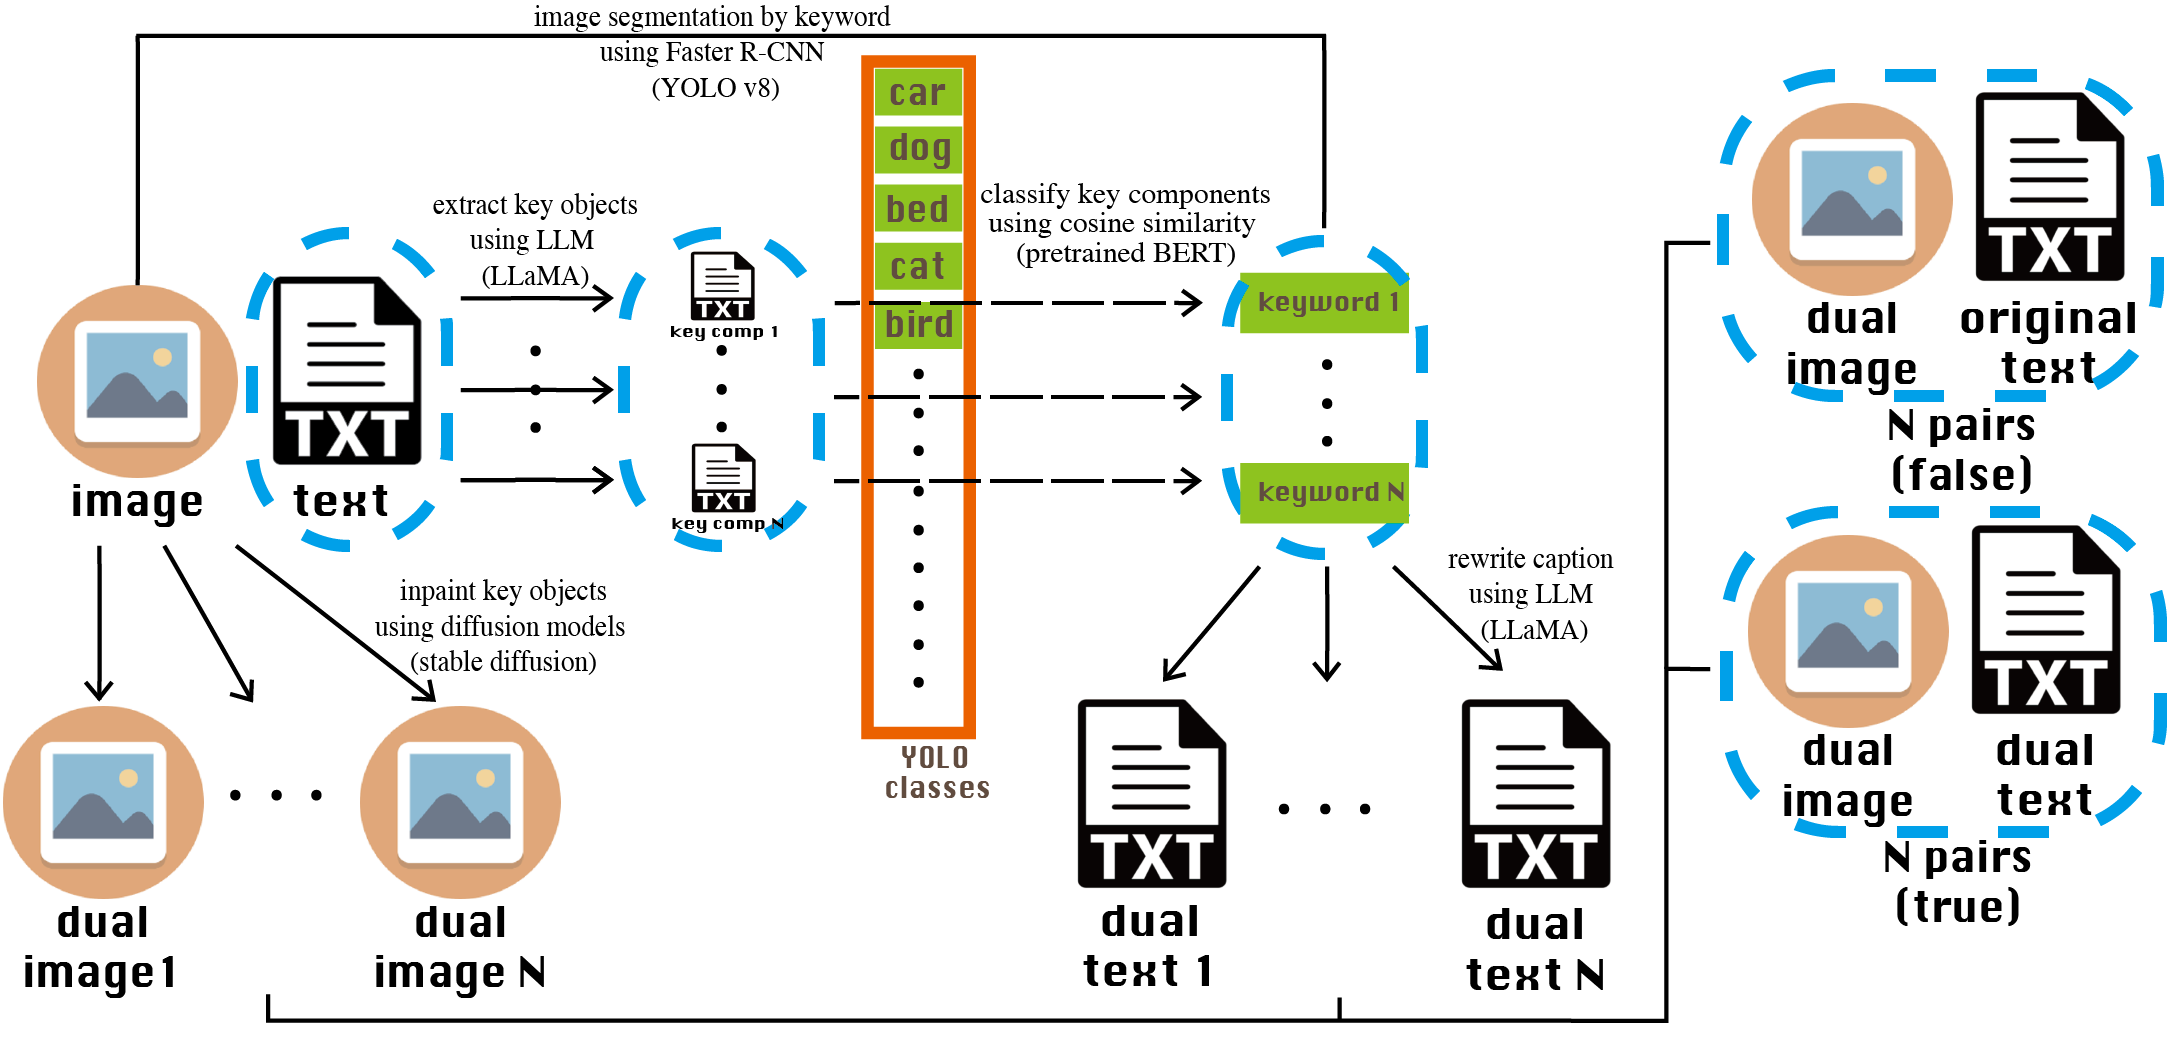
\includegraphics[width=1\textwidth]{midterm_report/assets/pipeline2.png}
    \caption{Overall approach}
\end{figure}
In concrete: 
\begin{itemize}
    \item We assign a small hyperparameter $N$ (e.g., $N=3$)
    \item Utilize the in-context learning capability of large language models to extract $N$ key components (if possible), and categorize them into a few pretrained classes.
    \item Perform image segmentation using Fast RCNN models (e.g., \texttt{YOLO v8}) to extract $N$ key components from the image, generate masks.
    \item Use diffusion model to do image inpaining, generating $N$ new images by respectively removing the $N$ components on the original image.
    \item Rewrite the original caption by LLM to remove each keyword from the text, and get $N$ dual texts accordingly.
\end{itemize}


\begin{figure}{H} % r: 图片在右侧
    \centering
    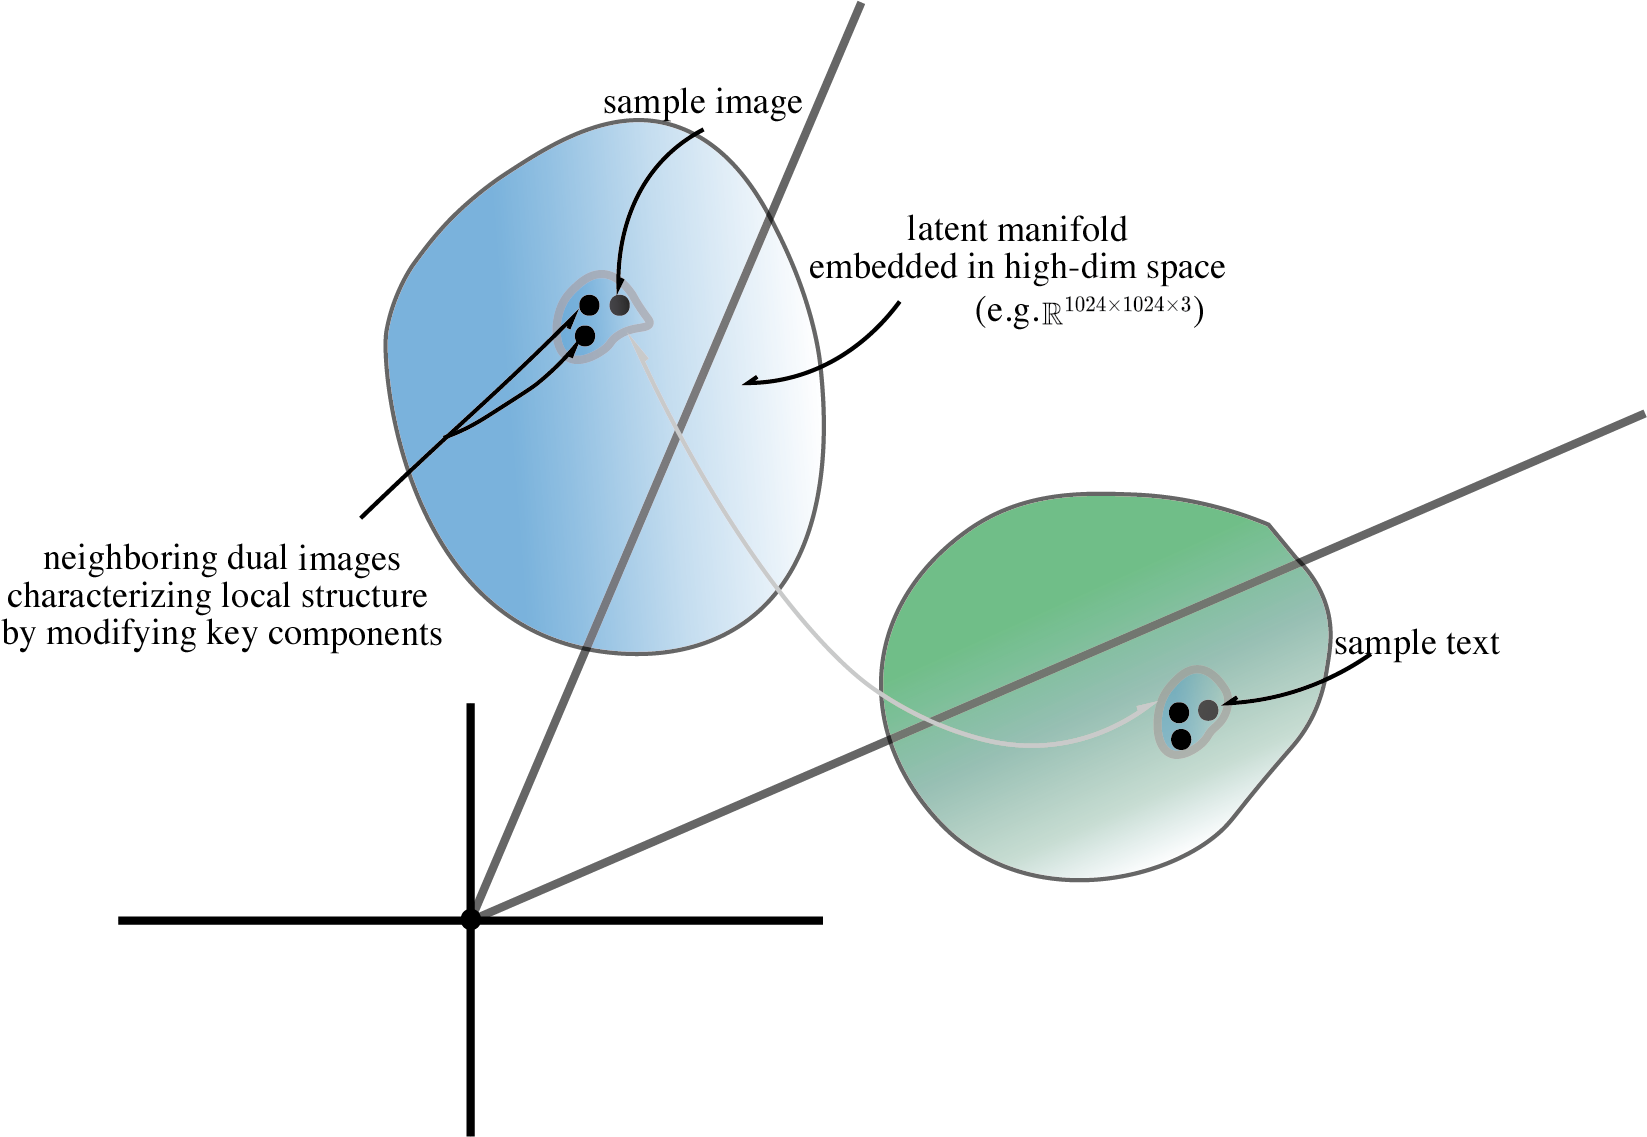
\includegraphics[width=0.7\textwidth]{midterm_report/assets/manifold.png}
    \caption{Embedding data manifold in Clip Space}
\end{figure}

Our idea invokes the manifold hypothesis, aims at improving CLIP's composition-reasoning ability. Prior work has shown that the embedding manifold of CLIP is characterized as double-ellipsoids\cite{levi2024doubleellipsoidgeometryclip} (Levi, Gilboa, 2024), and we hypothesize: dual images with critical components removed characterize the local structure of the original image, as a valid interpolation; and the generation of dual texts can let the model learn the mapping between the sample image and the open neighborhood near the caption. We conjecture that our approach increases the combinatorial inference ability and robustness of the model on training with small datasets.




\begin{comment}
  \begin{center}
    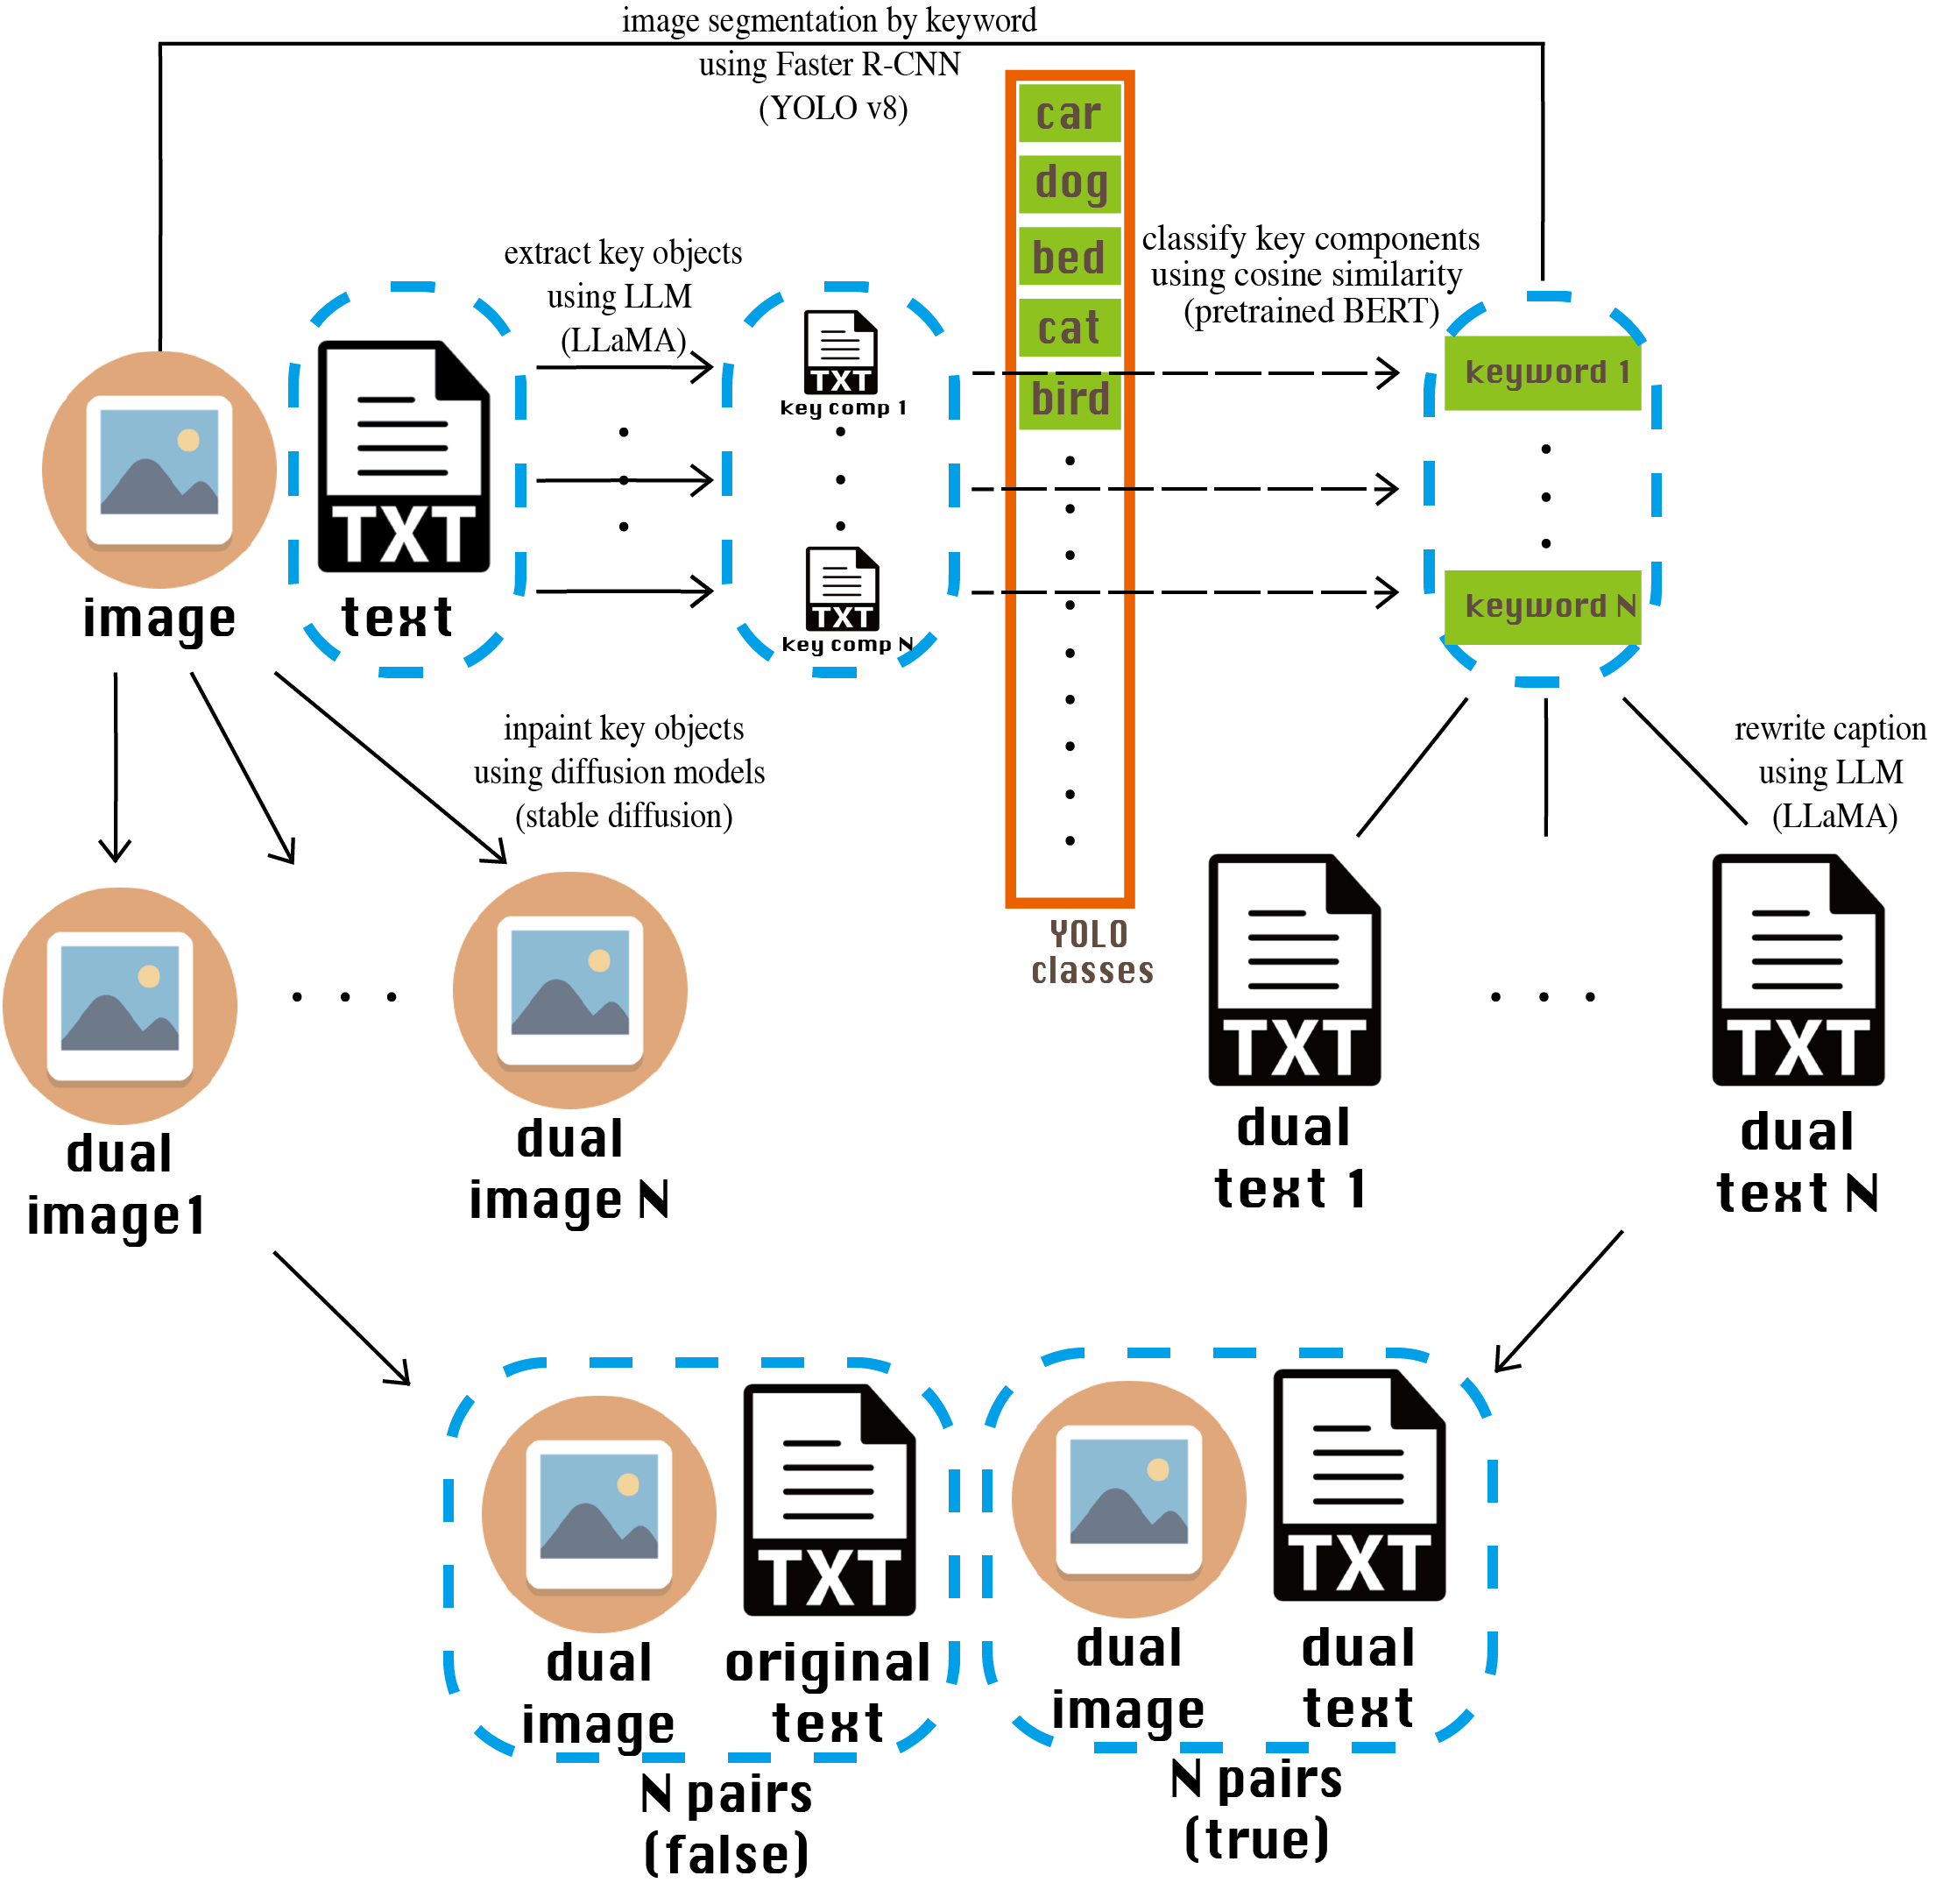
\includegraphics[width=1\textwidth]{midterm_report/pipeline.png} 
\end{center}
\end{comment}




\section{Related work}
\subsection{Existing Methods:}
 CLIP's performance is shown recently that it could be enhanced by leverging the difficulty in training.\\
Currently the exisiting methods mostly improve in the following perspectives.\\
\begin{itemize}
    % \item \textbf{Hard Negative Mining}: Hard negative examples are those that are semantically similar to the positive samples but belong to different classes, making it challenging for the model to distinguish between them. In contrastive learning, two primary strategies enhance model performance: generation-based methods and regularization-based methods. Generation-based methods, such as NegCLIP and SVLC, create hard negatives by altering positive samples to produce semantically similar yet incorrect pairs, challenging models to discern subtle differences. Regularization-based methods employ strategies like intra-modal contrastive loss and ranking cross-modal hard negatives to refine learning.

    \item \textbf{Hard Negative Mining}: Hard negatives closely resemble positive samples yet belong to different classes, making them difficult to distinguish. In contrastive learning, two main strategies address this: generation-based and regularization-based. Generation-based methods (e.g., NegCLIP\cite{yuksekgonul2023visionlanguagemodelsbehavelike} ((Yuksekgonul et al., 2022)) modify positive samples to create semantically similar but incorrect pairs, forcing models to learn subtle distinctions. Regularization-based methods use techniques like intra-modal contrastive loss and cross-modal ranking of hard negatives to refine learning.

    
    
    \item \textbf{Fine-Grained Cross-Modal Alignment Fine-Tuning}: Some previous works such as FILIP\cite{yao2021filipfinegrainedinteractivelanguageimage} (Yao et al., 2021) enhances multimodal alignment by matching local image patches with specific text tokens via a similarity matrix. Unlike CLIP’s global image-text matching, it computes token-level contrastive losses, forcing visual and textual tokens to mutually select their most relevant counterparts. The regional information and details could be better learned this way.
    \item \textbf{Rewrite Empowered by Large Language Model}: LaCLIP\cite{fan2023improvingcliptraininglanguage} ((Fan, Krishnan, et. al) generates diverse text rewrites for each image caption via LLMs while preserving semantic meaning, boosting the performances significantly on datsets such as  CC12M and LAION-400M . 
\end{itemize}
\subsection{Comparisons:}
DeCLIP combines the idea of \textbf{Hard Negative Mining} and \textbf{Fine-Grained Cross-Modal Alignment Fine-Tuning} such that the model can deepen its understanding of the entire image by paying attention to the regional changes of the image. From the proposed method section, DeCLIP uses Large language model to capture keywords from the caption in the data set and replaces those keywords one at a time with pre-trained catogeries, forming our final traning set. It is different from \textbf{Hard Negative Mining} in applying the changes to \textbf{images} instead of \textbf{texts}, while it is improved based on \textbf{Fine-Grained Cross-Modal Alignment Fine-Tuning} by considering contexts of texts and layout of images
\subsection{Core Model and Tool References:}
Our framework integrates state-of-the-art multimodal tools. For text extraction, \texttt{spaCy} \cite{spacy2025} identifies and merges compound nouns. We then map these nouns to pre-trained categories via \texttt{word2vec-google-news-300} embeddings. For image segmentation, \texttt{yolov8n-seg.pt} (a lightweight YOLOv8 variant pretrained on COCO) is used.\\ Inpainting leverages \texttt{runwayml/stable-diffusion-inpainting} and \texttt{CLIP}, ensuring robust image–text understanding.





\section{Preliminary}


\section*{Pipeline for Caption-Guided Object Removal in Images}

We have completed a pipeline that uses the image caption to guide the removal of specific objects. Currently, our system operates on a single image--caption pair. The code is provided in the Appendix A.

\subsection*{Example}
\noindent
   \begin{figure}[h]
    \centering
    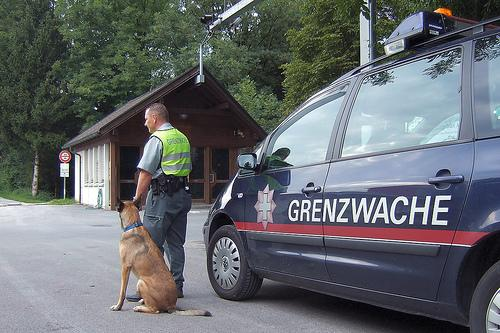
\includegraphics[width=0.3\textwidth]{midterm_report/assets/oriIMG.jpg}
    \caption{\textcolor{blue}{\textbf{Caption:} \emph{``A policeman stops on a street with a search dog.''}}}
    \label{fig:original_image}
\end{figure}
\subsubsection*{Step 1: Extraction of Nouns/Noun Phrases}

\textbf{Method:} We use SpaCy's small English language model to extract nouns and noun phrases from the caption. For compound phrases such as ``search dog,'' the entire phrase is treated as a single unit.

\noindent
\textbf{Example:}
\begin{itemize}
  \item \textcolor{blue}{ Extracted Terms: ``policeman'', ``street'', ``search dog''}
\end{itemize}


\subsubsection*{Step 2: Classification into Object Categories}

\textbf{Method:}The extracted noun phrases are mapped to one of the 80 object classes used by YOLOv8. Mapping is achieved using a pre-trained Word2Vec model.


\noindent
\textbf{Example:}
\textcolor{blue}{\begin{itemize}
  \item \texttt{policeman} $\to$ \texttt{person |}
  \texttt{street} $\to$ \texttt{bicycle |}
  \texttt{search dog} $\to$ \texttt{dog}
\end{itemize}}

\noindent
Ambiguous mappings (like ``street'') are discarded later if they do not appear in the detection step. When dealing with phrases like ``search dog,'' we ensure that word phrases are considered based on the weight of each word.



\subsubsection*{Step 3: Object Detection and Mask Generation}

\noindent
\textbf{Method:} \\
YOLOv8 is applied to the image to detect each of the classified objects. If an object is not detected, it is discarded from the pipeline. For each detected object, a binary mask is generated—white for the object and black for the background.

\noindent
\textbf{Example:}
\begin{figure}[h]
    \centering
    \begin{subfigure}[b]{0.2\textwidth}
        \centering
        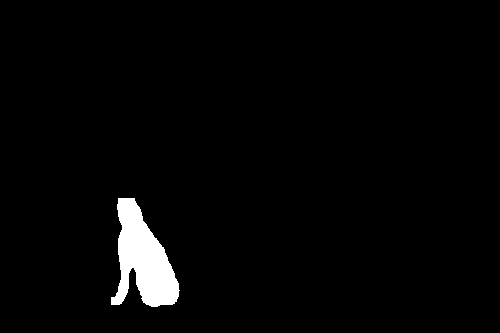
\includegraphics[width=\textwidth]{midterm_report/assets/dogMask.jpg}
        \caption{\textcolor{blue}{\textbf{Mask for Dog}}}
        \label{fig:mask_dog}
    \end{subfigure}
    \hfill
    \begin{subfigure}[b]{0.2\textwidth}
        \centering
        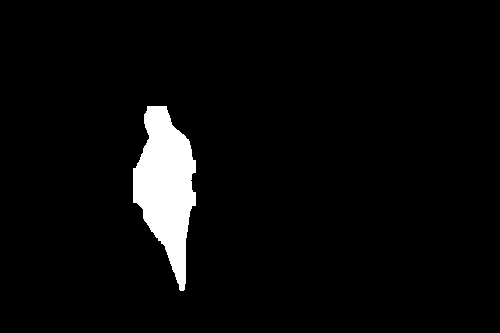
\includegraphics[width=\textwidth]{midterm_report/assets/PersonMask.jpg}
        \caption{\textcolor{blue}{\textbf{Mask for Person}}}
        \label{fig:mask_person}
    \end{subfigure}
    \caption{Binary masks for detected objects. The bicycle was discarded.}
    \label{fig:mask_comparison}
\end{figure}

\subsubsection*{Step 4: Object Removal via Inpainting}

\noindent
\textbf{Method:} \\
We use a Stable Diffusion inpainting model to remove each detected object using its corresponding binary mask. This process is guided by a prompt such as: \emph{``Only blend the highlighted block seamlessly into the background.''}

\noindent
\textbf{Example:}
\begin{figure}[h]
    \centering
    \begin{subfigure}[b]{0.2\textwidth}
        \centering
        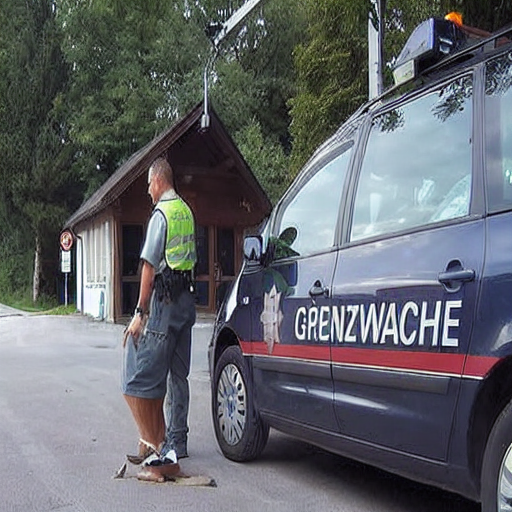
\includegraphics[width=\textwidth]{midterm_report/assets/output_dog.png}
        \caption{Inpainted Output (Dog Removed)}
        \label{fig:inpaint_dog}
    \end{subfigure}
    \hfill
    \begin{subfigure}[b]{0.2\textwidth}
        \centering
        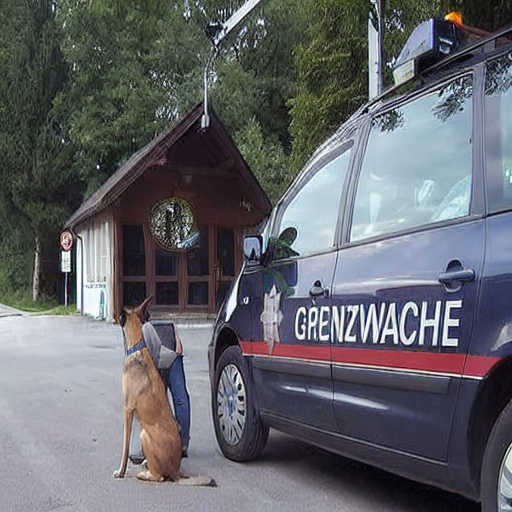
\includegraphics[width=\textwidth]{midterm_report/assets/output_person (1).png}
        \caption{Inpainted Output (Person Removed)}
        \label{fig:inpaint_person}
    \end{subfigure}
    \caption{Inpainting results after object removal. The bicycle was discarded.}
    \label{fig:inpaint_comparison}
\end{figure}

\noindent
\textbf{Future Work:} \\
Removing multiple objects in a single mask is a straightforward extension of this approach.

\noindent
\textbf{Challenges:}
\begin{enumerate}
    \item \textbf{Key Noun Extraction:} Initial attempts using large language models (e.g., GPT, LLaMA) were unsatisfactory. We opted to extract \emph{all} nouns instead. Future work may explore random selection.
    \item \textbf{Classification Difficulties:} BERT-based methods (even with the entire-caption context) did not yield accurate classifications.
    \item \textbf{Bounding Box Precision:} Early tests using rectangular bounding boxes led to imprecise masks. More precise detection methods now provide smoother, more accurate masks.
\end{enumerate}



\section{Conclusion}
In this work, we developed a caption-guided object removal pipeline that leverages YOLOv8-based object detection, stable diffusion inpainting, and large language models to extract key objects from image-caption pairs, classify them into predefined categories, and generate precise masks for targeted object removal. By modifying images, while preserving structural relevance, we created hard negative images that misalign with their original captions, enhancing contrastive learning in CLIP-based models and improving their ability to distinguish fine-grained differences between text and images. Additionally, the altered images were incorporated into the training dataset as false samples to find tune the existing model. While our approach demonstrates the feasibility, future work should focus on refining object classification, supporting multi-object handling, and scaling data generation to improve DeClip’s effectiveness in multimodal learning.

\section{Future Plan}
\begin{itemize}
    \item We will need to automate the procedure for relatively large dataset (e.g. 3 million images), requiring the balance between efficiency and quality of inpainting, otherwise we might introduce noisy generated images. So we may need to tweak the tech stack and architecture slightly after practice.
    \item We will further optimize the structure: if a class of examples are already well-learned, then we do not need to improve the accuracy of shotting concerning images. We will not generate $2N$ new examples for all existing examples, but reselect a subset of all images in a dataset for computation cost.
\end{itemize}

\section{Contributors and Roles}
\begin{itemize}
    \item \textbf{Zhanhao Liu} 
    \begin{itemize}
        \item Authored the \emph{Preliminary Section} of the report.
        \item Implemented the \emph{word matching} and \emph{Stable Diffusion} code.
    \end{itemize}
    \item \textbf{Huanchen Jia} 
    \begin{itemize}
        \item Authored the \emph{Related Work} section of the report.
        \item Researched state-of-the-art methods and reviewed the literatures for the group.
        \item Implemented the \emph{noun extraction} and \emph{compound word emerging} code.
    \end{itemize}
    \item \textbf{Qiulin Fan} 
    \begin{itemize}
        \item Conceived the idea.
        \item Authored the \emph{Proposed Method} section of the report.
        \item Implemented the \emph{object detection and mask generation} code.
    \end{itemize}
    \item \textbf{Lingyu Meng} 
    \begin{itemize}
        \item Researched \emph{datasets and benchmarks} for future work.
        \item Authored the \emph{Introduction} and \emph{Conclusion} sections of the report.
    \end{itemize}
\end{itemize}

\printbibliography


\appendix
\section*{Appendix A: Code}
\addcontentsline{toc}{section}{Appendix A: Proposed Datasets}

\begin{lstlisting}[language=Python, caption={Code for Noun extraction}, label={lst:mask_processing}]
import spacy
from collections import Counter
nlp = spacy.load("en_core_web_sm")
def extract_nouns(sentence, top_n=5):
    doc = nlp(sentence)

    # Merge consecutive nouns into phrases (e.g., "plant species")
    phrases = []
    current_phrase = []
    for token in doc:
        if token.pos_ in ['NOUN', 'PROPN']:
            current_phrase.append(token.text)
        else:
            if current_phrase:
                phrases.append(" ".join(current_phrase))
                current_phrase = []
    # Process any remaining noun phrase
    if current_phrase:
        phrases.append(" ".join(current_phrase))

    # Count phrase frequency
    counts = Counter(phrases)
    return [phrase for phrase, _ in counts.most_common(top_n)]

sentence = "A policeman stops on a street with a search dog."
list_A = extract_nouns(sentence)
print("Extracted nouns/phrases:", list_A)
\end{lstlisting}

\begin{lstlisting}[language=Python, caption={Code for words match}, label={lst:mask_processing}]
import numpy as np
from sklearn.metrics.pairwise import cosine_similarity
from gensim.models import KeyedVectors

# Predefined YOLO keywords
YOLOKeyWords = [
    "person", "bicycle", "car", 
    # ...
    "vase", "scissors", "teddy bear",
    "hair drier", "toothbrush"
]

# Load the Word2Vec model (Google News vectors)
model = api.load("word2vec-google-news-300")

def get_phrase_vector(phrase, model):
    tokens = phrase.split()  # Basic whitespace split
    token_vectors = []
    for token in tokens:
        try:
            token_vectors.append(model[token])
        except KeyError:
            print(f"Token '{token}' not found in vocabulary; skipping.")
    if token_vectors:
        return np.mean(token_vectors, axis=0)
    else:
        print("No valid tokens found in the phrase.")
        return None

def classify_word_by_similarity(phrase, class_words, model, threshold=0.0):
    phrase_vector = get_phrase_vector(phrase, model)
    if phrase_vector is None:
        return None

    class_vectors = []
    valid_class_words = []
    for w in class_words:
        try:
            vec = model[w]
            class_vectors.append(vec)
            valid_class_words.append(w)
        except KeyError:
            continue
    
    if not class_vectors:
        return None

    class_vectors = np.array(class_vectors)
    similarities = cosine_similarity(phrase_vector.reshape(1, -1), class_vectors).flatten()
    best_index = np.argmax(similarities)
    best_similarity = similarities[best_index]

    if best_similarity < threshold:
        return None
    return valid_class_words[best_index], best_similarity

# Example usage
# word = "policeman"
# result = classify_word_by_similarity(word, YOLOKeyWords, model, threshold=0.3)
# print("Nearest-Neighbor Class:", result)

# Classify a list of words
keywords = []
print(list_A)
for word in list_A:
    result = classify_word_by_similarity(word, YOLOKeyWords, model, threshold=0.3)
    if result:
        keywords.append(result[0])

print(keywords)
\end{lstlisting}

\begin{lstlisting}[language=Python, caption={Code for Object detection and mask generation}, label={lst:mask_processing}]
# @title YOLO
from ultralytics import YOLO
import cv2
import numpy as np
import os

# Load YOLO model
model = YOLO("yolov8n-seg.pt")

# Detect and segment objects in the input image
results = model(input_image_path)
img = cv2.imread(input_image_path)
height, width = img.shape[:2]

# Initialize dictionary to store combined masks for each keyword
combined_masks = {k: np.zeros((height, width), dtype=np.uint8) for k in keywords}
label_detected = []

# Iterate over detection results and extract segmentation masks
for result in results:
    if result.masks is not None:
        for i in range(len(result.boxes)):
            class_id = int(result.boxes.cls[i])
            label = model.names[class_id]
            if label in keywords:
                label_detected.append(label)
                
                # Extract mask and binarize
                mask = result.masks.data[i].cpu().numpy()
                mask = (mask > 0.2).astype(np.uint8) * 255
                
                # Resize if necessary
                if mask.shape[0] != height or mask.shape[1] != width:
                    mask = cv2.resize(mask, (width, height), interpolation=cv2.INTER_NEAREST)
                
                # Combine masks for the same label
                combined_masks[label] = cv2.bitwise_or(combined_masks[label], mask)

# Save each mask to the specified folder
maskFolder = "maskFolder"
os.makedirs(maskFolder, exist_ok=True)

for label, mask in combined_masks.items():
    mask_path = f"mask_{label}.png"
    output_image_path = os.path.join(maskFolder, mask_path)
    cv2.imwrite(output_image_path, mask)
    print(f"Saved mask for '{label}' as {output_image_path}")
\end{lstlisting}

\begin{lstlisting}[language=Python, caption={Code for Noun extraction}, label={lst:mask_processing}]
# @title Stable Diffusion
from diffusers import StableDiffusionInpaintPipeline
import torch
from PIL import Image
import os

# Load the inpainting model
model_id = "runwayml/stable-diffusion-inpainting"
pipe = StableDiffusionInpaintPipeline.from_pretrained(
    model_id, torch_dtype=torch.float16
)

# Set device
device = "cuda" if torch.cuda.is_available() else "cpu"
pipe = pipe.to(device)

# Load input image
input_image_path = "image.png"  # Replace with your actual image path
image = Image.open(input_image_path).convert("RGB")

# Ensure the output directory exists
outputfolder = "OutputFolder"
os.makedirs(outputfolder, exist_ok=True)

# Process each detected label
for label in label_detected:
    # Load corresponding mask
    mask_path = os.path.join(maskFolder, f"mask_{label}.png")
    mask = Image.open(mask_path).convert("RGB")
    
    # Define output path
    output_image_path = os.path.join(outputfolder, f"output_{label}.png")
    
    # Perform inpainting
    result = pipe(prompt=prompt, image=image, mask_image=mask).images[0]
    
    # Save the result
    result.save(output_image_path)
    print(f"Saved inpainted image for '{label}' as {output_image_path}")
\end{lstlisting}
\end{document}